% !TEX root = ../../presentation.tex
% Meta: Vision

\begin{slide}{Vision}
  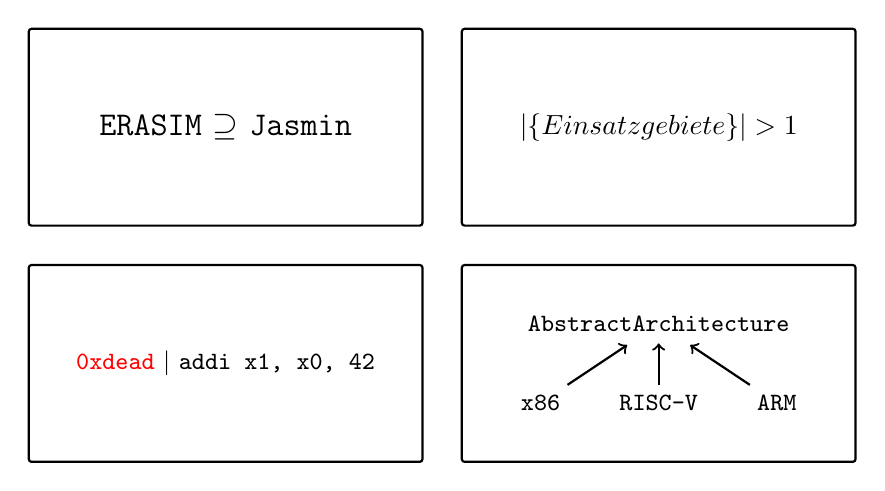
\begin{tikzpicture}[thick, rounded corners=1pt]
    \onslide<2->{
    \draw (0, 0) rectangle ++(5, 2.5)
          node [midway, align=center]
          {\large\texttt{ERASIM} $\supseteq$ \texttt{Jasmin}};
    }

    \onslide<3->{
    \draw (5.5, 0) rectangle ++(5, 2.5)
          node [midway, align=center] {$|\{\text{Einsatzgebiete}\}| > 1$};
    }

    \onslide<4->{
    \draw (0, -3) rectangle ++(5, 2.5)
          node [midway, align=center]
        {\small \textcolor{Red}{\texttt{0xdead}} $|$ \texttt{addi x1, x0, 42}};
    }

    \onslide<5->{
    \draw (5.5, -3) rectangle ++(5, 2.5);
    \node (arch) at (8, -1.25) {\small\texttt{AbstractArchitecture}};
    \node (x86) at (6.5, -2.25) {\small\texttt{x86}};
    \node (riscv) at (8, -2.25) {\small\texttt{RISC-V}};
    \node (arm) at (9.5, -2.25) {\small\texttt{ARM}};

    \draw [->, shorten >= 2pt] (x86) -- (arch);
    \draw [->, shorten >= 0.5pt] (riscv) -- (arch);
    \draw [->, shorten >= 2pt] (arm) -- (arch);
    }
  \end{tikzpicture}
\end{slide}

% \begin{slide}{Vision}
%   \Large
%   \vspace{0.5cm}
%   $\text{Erweiterbarkeit}: \text{Zeit} \rightarrow \text{Features}$
%
%   \vspace{1cm}
%   \texttt{(ERASIM)}
% \end{slide}
%
% \begin{slide}{Vision}
%   \Large
%   \vspace{0.5cm}
%   $\text{Erweiterbarkeit}: \text{Zeit} \times \text{Neues Design} \rightarrow \text{Features}$
%
%   \vspace{1cm}
%   \texttt{(JASMIN)}
% \end{slide}
